\documentclass[12pt,a4paper,bibliography=totocnumbered,listof=totocnumbered]{scrartcl}
\usepackage[ngerman]{babel}
\usepackage[utf8]{inputenc}
\usepackage{amsmath}
\usepackage{amsfonts}
\usepackage{amssymb}
\usepackage{graphicx}
\usepackage{fancyhdr}
\usepackage{tabularx}
\usepackage{geometry}
\usepackage{setspace}
\usepackage{xcolor}
\usepackage[right]{eurosym}
\usepackage[printonlyused]{acronym}
\usepackage{subfig}
\usepackage{floatflt}
\PassOptionsToPackage{usenames,dvipsnames}{color}
\usepackage{colortbl}
\usepackage{paralist}
\usepackage{array}
\usepackage{titlesec}
\usepackage{parskip}
\usepackage[right]{eurosym}
\usepackage{picins}
\usepackage{textcomp} % Eurozeichen und andere Symbole
\usepackage{xspace} % Leerzeichen nach LaTeX -Befehlen
\usepackage[subfigure,titles]{tocloft}
\usepackage[pdfpagelabels=true]{hyperref}
\usepackage[babel,german=quotes]{csquotes}
\usepackage{romannum}
\usepackage{enumitem} % Konfigurierbare Aufzählungen und Listen
\usepackage{array} % Erweiterungen für Tabellen
\usepackage{tabu} % Erweiterte Formatierung in Tabellen
\usepackage{wrapfig} % von Text umflossene Elemente
\usepackage{dirtree}

\usepackage[
	backend=biber,
	style=alphabetic,
	citestyle=alphabetic,
	sorting=nty,
	doi=true,url=true,
]{biblatex}
\bibliography{bib}

\usepackage{listings}
%\lstset{basicstyle=\footnotesize, captionpos=b, breaklines=true, showstringspaces=false, tabsize=2, frame=lines, numbers=left, numberstyle=\tiny, xleftmargin=2em, framexleftmargin=2em}
%\makeatletter
%\def\l@lstlisting#1#2{\@dottedtocline{1}{0em}{1em}{\hspace{1,5em} Lst. #1}{#2}}
%\makeatother

\lstset{
	basicstyle=\footnotesize\ttfamily,	% default font
	numbers=left,						% line numbers placement
	numberstyle=\tiny,					% line numbers style
	%stepnumber=2,						% line number padding
	numbersep=5pt,						% padding between line numbers and code
	tabsize=2,							% 
	extendedchars=true,         
	breaklines=true,					% line breaks 
	keywordstyle=\color{red},
%	frame=b,
	stringstyle=\color{gray}\ttfamily,	% color of strings in code
	showspaces=false,					% visualize spaces
    showtabs=false,						% visualize tabs
    xleftmargin=17pt,
	framexleftmargin=17pt,
	framexrightmargin=5pt,
	framexbottommargin=4pt,
	captionpos=b,
	frame=single,
	showstringspaces=false				% visualize spaces in strings        
 }
 
 \lstloadlanguages{% Check docs for further languages ...
         C,
         C++,
         bash,
         HTML,
         Java,
         Clean % use this for CSS
 }

\geometry{a4paper, top=27mm, left=30mm, right=20mm, bottom=35mm, headsep=10mm, footskip=12mm}

\hypersetup{unicode=false, pdftoolbar=true, pdfmenubar=true, pdffitwindow=false, pdfstartview={FitH},
%	pdftitle={Abschlussarbeit}, 
%	pdfauthor={Daniel Brettschneider},
%	pdfsubject={Abschlussarbeit},
%	pdfcreator={\LaTeX\ with package \flqq hyperref\frqq},
%	pdfproducer={pdfTeX \the\pdftexversion.\pdftexrevision},
%	pdfkeywords={Abschlussarbeit},
%	pdfnewwindow=true,
	colorlinks=true,linkcolor=black,citecolor=black,filecolor=magenta,urlcolor=black}
%\pdfinfo{/CreationDate (D:20110620133321)}

% Schriftart auf Helvetica ändern
\usepackage{helvet}
\renewcommand{\familydefault}{\sfdefault}
\fontfamily{phv}\selectfont

% Hurenkinder und Schusterjungen verhindern
\clubpenalty10000
\widowpenalty10000
\displaywidowpenalty=10000

% Benutzerdefinierte Befehle für späteren Werteabruf
\def\title#1{\gdef\@title{#1}\gdef\THETITLE{#1}}
\def\author#1{\gdef\@author{#1}\gdef\THEAUTHOR{#1}}
\newcommand{\authoremail}{\href{mailto:\email}{\email}}

% Wertezuweisung in Variablen, damit diese nur an einer Stelle geändert werden müssen
\title{Entwicklung eines Android Usability Testing Frameworks}
\author{Albert Hoffmann}
\newcommand{\email}{albert.hoffmann@hs-osnabrueck.de}
\newcommand{\pruefer}{Prof. Michaela Ramm, M.A.}

\begin{document}

\titlespacing{\section}{0pt}{12pt plus 4pt minus 2pt}{-6pt plus 2pt minus 2pt}

% Kopf- und Fusszeile
\renewcommand{\sectionmark}[1]{\markright{#1}}
\renewcommand{\leftmark}{\rightmark}
\pagestyle{fancy}
\lhead{}
\chead{}
\rhead{\thesection\space\contentsname}
\lfoot{\THETITLE}
\cfoot{}
\rfoot{\thepage}
\renewcommand{\headrulewidth}{0.4pt}
\renewcommand{\footrulewidth}{0.4pt}

% Vorspann
\renewcommand{\thesection}{\Roman{section}}
\renewcommand{\theHsection}{\Roman{section}}
\pagenumbering{Roman}

% ----------------------------------------------------------------------------------------------------------
% Titelseite
% ----------------------------------------------------------------------------------------------------------


\thispagestyle{empty}
\begin{center}
	
\includegraphics[scale=1]{img/hs_os}\\
	\vspace*{2cm}
	\Large
	\textbf{Fakultät}\\
	\textbf{Ingenieurwissenschaften und Informatik}\\
	\vspace*{2cm}
	\Huge
	\textbf{Projektdokumentation}\\
	\vspace*{0.5cm}
	\large
	für das \\
	\textbf{Masterprojekt}\\  
	mit dem Thema\\
	\vspace*{1cm}
	\textbf{\THETITLE}\\
	\vspace*{2cm}
	
	\vfill
	\normalsize
	\newcolumntype{x}[1]{>{\raggedleft\arraybackslash\hspace{0pt}}p{#1}}
	\begin{tabular}{x{6cm}p{7.5cm}}
		\rule{0mm}{5ex}\textbf{Autor:} & \THEAUTHOR \newline 
		\authoremail \\ 
		\rule{0mm}{5ex}\textbf{Prüfer:} & \pruefer \\ 
		\rule{0mm}{5ex}\textbf{Abgabedatum:} & 06.10.2014 \\ 
	\end{tabular} 
\end{center}
\pagebreak


\begin{abstract}

\noindent\textbf{Zusammenfassung:}\\ \\
Die vorliegende Ausarbeitung wurde in \LaTeX verfasst und ist eine gemeinsame Arbeit von Albert Hoffmann und Oliver Erxleben an der Hochschule Osnabrück / University of Applied Sciences im Masterstudiengang Informatik - Mobile und Verteilte Anwendungen des Fachbereichs Ingenieurswissenschaften und Informatik für das Modul Mensch-Maschine-Kommunikation im Wintersemester 2013/14. Die Arbeit dokumentiert die Entwicklung einer Programmierbibliothek zum Test der Usability von Mobilanwendungen für das Android-Betriebssystem.\\ \\
Die Arbeit gliedert sich in verschiedene Teile.\\
%TODO: update Aufbau und Ablauf
\end{abstract}
% Verzeichnisse
% ----------------------------------------------------------------------------------------------------------
% Verzeichnisse
% ----------------------------------------------------------------------------------------------------------
% TODO Typ vor Nummer
\renewcommand{\cfttabpresnum}{Tab. }
\renewcommand{\cftfigpresnum}{Abb. }
\settowidth{\cfttabnumwidth}{Abb. 10\quad}
\settowidth{\cftfignumwidth}{Abb. 10\quad}

\titlespacing{\section}{0pt}{12pt plus 4pt minus 2pt}{2pt plus 2pt minus 2pt}
\singlespacing
\rhead{INHALTSVERZEICHNIS}
\renewcommand{\contentsname}{II Inhaltsverzeichnis}
\phantomsection
\addcontentsline{toc}{section}{\texorpdfstring{II \hspace{0.35em}Inhaltsverzeichnis}{Inhaltsverzeichnis}}
\addtocounter{section}{1}
\tableofcontents
\pagebreak
\rhead{VERZEICHNISSE}
\listoffigures
\pagebreak
\listoftables
%\pagebreak
\renewcommand{\lstlistlistingname}{Listing-Verzeichnis}
{\labelsep2cm\lstlistoflistings}
\pagebreak
% ----------------------------------------------------------------------------------------------------------
% Abkürzungen
% ----------------------------------------------------------------------------------------------------------
\section{Abkürzungsverzeichnis}
%TODO: längste Abkürzung steht in eckigen Klammern
\begin{acronym}[HATEOAS]
\setlength{\itemsep}{-\parsep} % geringerer Zeilenabstand
\acro{OSGi}{Open Service Gateway initiative} %TODO entfernen
\acro{HTTP}{Hypertext Transfer Protocol}
\acro{SSL}{Secure Sockets Layer}
\acro{TLS}{Transport Layer Security}
\acro{UI}{User Interface}
\acro{JSON}{JavaScript Object Notation}
\acro{UX}{User Experience}
\acro{SDK}{Software Development Kit}
\acro{IDE}{Integrated Development Environment}
\acro{API}{Application Programming Interface}
\acro{NPM}{Node Package Manager}
\acro{VM}{Virtuelle Maschine}
\acro{SSH}{Secure Shell}
\acro{JAR}{Java Archive File}
\acro{CSS}{Cascading Style Sheets}
\acro{SQL}{Structured Query Language}
\acro{ER}{Entity Relationship}
\acro{REST}{Representational State Transfer}
\acro{URL}{Uniform Resource Locator}
\acro{SHA}{Secure Hash Algorithm}
\acro{AES}{Advanced Encryption Standard}
\acro{AS}{Application Server}
\acro{JPA}{Java Persistence API}
\acro{DBMS}{Database Management System}
\acro{JDBC}{Java Database Connectivity}
\acro{JAX-RS}{Java API for RESTful Web Services}
\acro{RPC}{Remote Procedure Call}
\acro{HATEOAS}{Hypermedia as the Engine of Application State}
\acro{CRUD}{Create, read, update and delete}
\acro{DAO}{Data Access Object}
\acroplural{DAO}[DAO's]{Data Access Objects}
\end{acronym}


% ----------------------------------------------------------------------------------------------------------
% Inhalt
% ----------------------------------------------------------------------------------------------------------
% Abstände Überschrift
%\titlespacing{\section}{0pt}{12pt plus 4pt minus 2pt}{-6pt plus 2pt minus 2pt}
%\titlespacing{\subsection}{0pt}{12pt plus 4pt minus 2pt}{-6pt plus 2pt minus 2pt}
%\titlespacing{\subsubsection}{0pt}{12pt plus 4pt minus 2pt}{-6pt plus 2pt minus 2pt}

% Kopfzeile
\renewcommand{\sectionmark}[1]{\markright{#1}}
\renewcommand{\subsectionmark}[1]{}
\renewcommand{\subsubsectionmark}[1]{}
\lhead{Kapitel \thesection}
\rhead{\rightmark}

\onehalfspacing
\renewcommand{\thesection}{\arabic{section}}
\renewcommand{\theHsection}{\arabic{section}}
\setcounter{section}{0}
\pagenumbering{arabic}
\setcounter{page}{1}


\section{Einleitung}
\subsection{Bezug der Programmquellen und Dokumentation}
Die Programmquellen der entwickelten, bzw. weiterentwickelten Software ist in dem folgenden \emph{GitHub}-Repository abrufbar:
\begin{center}
	\url{https://github.com/Chromdioxyde/hipsterbility}
\end{center}
Als Versionsverwaltung wird \emph{Git}\footnote{Git Webseite: \url{http://git-scm.com/}} eingesetzt.
Mit dem Befehl
\\
 \texttt{git clone https://github.com/Chromdioxyde/hipsterbility.git} kann eine lokale Kopie erstellt werden.
Alternativ kann der Inhalt des Repositories auf der o.~g. Webseite auch als ZIP-Datei heruntergeladen werden.
Die Quellen der Programme liegen im \emph{IntelliJ IDEA}\footnote{IntelliJ IDEA Website: \url{https://www.jetbrains.com/idea/}} Projektformat vor.
Für die Entwicklung wurde \emph{IntelliJ IDEA Ultimate 13.1.5} verwendet.

\subsection{Motivation}
Bei begrenztem Budget, z.~B. von Studierenden sind umfangreiche Labortests oder das Beauftragen von Dienstleistern oft nicht möglich.

Ein weiterer Faktor ist auch die Zielgruppe für die entwickelte Anwendung.
Bei räumlich verteilten Anwendern sind Labortests durch den logistischen Aufwand nur schwer möglich und auch die finanzielle Belastung steigt durch Transportkosten und evtl. mobiles Equipment.

Deshalb wurde im Wintersemester 2013/2014, zusammen mit Oliver Erxleben, ein Projekt durchgeführt, mit dem Ziel Usability-Tests mit minimalem Aufwand für den Teilnehmer durchzuführen (siehe Abschnitt \ref{subsec:stand_bei_projektbeginn}).

Die damals gesammelten Erkenntnisse und Erfahrungen sollen nun vertieft werden, mit dem Ziel die bestehenden Prototypen zu einem nutzbaren Framework weiter zu entwickeln.


\subsection{Zielsetzung}
Das Ziel ist es, ein Usability-Testing Framework oder Toolkit zu entwickeln, mit dem auch einzelne Entwickler oder kleine Teams ihre Anwendungen und Prototypen mit der Hilfe von Testbenutzern testen können.
Für den eigentlichen Testablauf beim Benutzers soll nur ein Android basiertes Gerät und eine Internetverbindung benötigt werden.
Ziel dabei ist es, das Testen möglichst einfach zu gestalten, ohne Labor und zusätzliches Equipment.

Auf der Seite des Testleiters soll nur ein PC oder Notebook benötigt werden, ohne zusätzliche Hardware.
Die Serverkomponente wurde ausgelagert, für den Fall, dass ein Server zur Verfügung steht, bzw. z.~B. von einer Bildungseinrichtung bereitgestellt wird.
\subsection{Problemstellung}
%TODO: Problemstellung
\subsection{Stand bei Projektbeginn\label{subsec:stand_bei_projektbeginn}}
Dieses Projekt basiert auf einer Arbeit, welche zusammen mit Oliver Erxleben (\href{mailto:oliver.erxleben@hs-osnabrueck.de}{oliver.erxleben@hs-osnabrueck.de}) im Modul \emph{Mensch-Maschine-Kommunikation} (Wintersemester 2013/2014) des Informatik--Masterstudiengangs \emph{Verteilte und mobile Anwendungen} erstellt wurde.
Die Ergebnisse zum Stand der Abgabe können aus dem Git-Repository von Oliver Erxleben unter der folgenden \ac{URL} abgerufen werden:

\url{https://github.com/olivererxleben/hipsterbility/releases/tag/v1.0_semester_final}

Der Vollständigkeit halber wird der Stand der vorausgehenden Arbeit an dieser Stelle kurz wiedergegeben.
Es wurde ein Prototyp erstellt, welcher aus einer Android Bibliothek und einem kleinen \ac{REST}-Server besteht.
Zum Testen der Bibliothek wurde weiterhin eine kleine Android Applikation erstellt.
Insgesamt wurde folgender Funktionsumfang skizziert:
\begin{compactitem}
	\item Android 4.x Bibliothek
	\begin{itemize}
		\item Abrufen von Testsitzungen und Testaufgaben vom Server.
		\item Benutzeroberfläche zum Auswählen und Starten von Testsitzungen.
		\item Aufzeichnen des Kamerabildes der Frontkamera mit Ton, nach dem Starten einer Testsitzung.
		\item Erstellen von Screenshots der Applikation bei Benutzereingaben auf dem Touchscreen und Visualisierung der Eingaben auf dem Screenshot.
		\item Hochladen der gesammelten Daten zum Server.
	\end{itemize}
	\item Node.js basierter Server mit REST-Schnittstelle und Webinterface
	\begin{itemize}
		\item Bereitstellen von Testsitzungen und -aufgaben.
		\item Rudimentäres Benutzermanagement.
		\item Weboberfläche zum Erstellen von Testsitzungen und -aufgaben
		\item Speichern der hochgeladenen Daten in einer Datenbank und im Dateisystem.
		\item Aufbereiten der Screenshots und des Videos von der Frontkamera in ein Ergebnisvideo für die Auswertung.
	\end{itemize}
\end{compactitem}

Die Idee und die ursprüngliche Planung stammen von Oliver Erxleben, welcher auch für die Serverkomponente zuständig war.

Da viele Funktionen in der Implementierung nur skizziert wurden eignet sich der Prototyp nicht für die Verwendung in einer produktiven Umgebung.

Folgende Komponenten wurden aus der vorhergehenden Arbeit übernommen und weiterentwickelt:
\begin{compactitem}
	\item das grundlegende Konzept,
	\item Teile des Datenmodells,
	\item und Quellen der Android Bibliothek und Testapplikation.
\end{compactitem}

Der Server wird auf der Basis von \emph{Java EE 7} neu aufgebaut.
%TODO: Querverweis

\section{Stand der Technik}\label{sec:stand_der_technik}
\subsection{Mobile Usability Labortests}
Usability-Tests können grob in zwei räumliche Kategorien eingeteilt werden, Labortests und Feldtests, welche jeweils moderiert oder unmoderiert stattfinden können.

Ein einfacher Testaufbau für Labortests lässt sich z.B. mit Hilfe eines Computers mit angeschlossener, externer Kamera realisiert werden. 
Vorausgesetzt werden auch entsprechende Räumlichkeiten und Benutzer, welche die Tests durchführen.
Die, an den Computer angeschlossene Kamera, dient zum Aufzeichnen und Dokumentieren des Bildschirms eines mobilen Gerätes auf dem getestet wird.
Über die Kamera werden auch die Benutzereingaben dokumentiert. \cite[Vgl.][]{Budiu.2014}
Dies ist ein Beispiel für gängige Labortests.
Testmethoden für Labortests werden an dieser Stelle nicht weiter behandelt.
Im nächsten Abschnitt werden zwei Anbieter für Remote Usability Tests vorgestellt.

\subsection{Remote Usability Testing Anbieter\label{subsec:usability_testing_anbieter}}
Neben Methoden und Werkzeugen zum Messen und Testen von Software-Usability gibt es auch Dienstleister, deren Geschäftsmodell auf Usability-Tests und Untersuchungen basiert.
Hier werden einige Anbieter solcher Dienstleister kurz vorgestellt und das Angebot kurz beschrieben.
Die Auswahl und Beschreibung beschränkt sich auf Anbieter, die das Testen von mobile Applikationen anbieten.

\subsubsection{UserTesting\label{subsubsec:usertesting}}
Der Dienstleister \emph{UserTesting} (\url{http://www.usertesting.com/}) bietet, unter anderem, Usability-Studien an, welche von Testteilnehmern durchlaufen werden.
Das Angebot beinhaltet auch das Testen von mobilen Webseiten und Applikationen. \cite[Vgl.][]{UserTesting.2014c}

Der Kunden/Auftraggeber stellt Testaufgaben zusammen, welche die Testpersonen erfüllen sollen.
Es gibt die Möglichkeit Geräteklasse, Anzahl der Testteilnehmer und eine Zielgruppe festzulegen.
Das Ergebnis der in Auftrag gegebenen Studie kann, laut Anbieter, schon nach ca. einer Stunde vorliegen und umfasst Videos von Testteilnehmern währen der Tests, schriftliche Antworten und die Möglichkeit der anschließenden Befragung der Teilnehmer. \cite[Vgl.][]{UserTesting.2014b}

Das Angebot zum Testen von mobilen Applikationen umfasst die Plattformen Android und iOS.
Pro Plattform werden als Testgeräte Tablets und Smartphones angeboten, welche bei der Spezifikation einer Teststudie angegeben werden. 
Auch hier werden Zielgruppen ausgewählt und Testaufgaben spezifiziert.
Das Testergebnis umfasst auch eine Videoaufzeichnung vom Test, auf dem der Gerätebildschirm sichtbar ist und der Benutzer Aussagen, z.~B. nach der \emph{Thinking Aloud} Methode, tätigt.
Die pauschalen Kosten für kleine Studien belaufen sich auf \$49 pro Testbenutzer.
\cite[Vgl.][]{UserTesting.2014}

\subsubsection{UserZoom \label{subsubsec:userzoom}}
Das \emph{UserZoom} (\url{http://www.userzoom.de}) Angebot vereint Werkzeuge und Dienstleistungen.
Letztere sind vorwiegend unterstützender Natur und umfassen z.B. Beratung, Rekrutierung von Teilnehmern und den Kunden-Support \cite[vgl.][]{UserZoomGmbH.2013b}.

Das Angebot bzgl. des Mobile Testing umfasst eine mobile Applikation für die iOS und Android Plattformen, welche sich zum Testen von Webseiten und webbasierten App-Prototypen eignet.
Das Verfahren wird als \enquote{[...] Remote Unmoderated Mobile Usability Testing [...]} \cite{UserZoomGmbH.2013c} bezeichnet und erlaubt ein standortunabhängiges Testen.
Angemeldete Testpersonen werden in Zielgruppen eingeteilt und per E-Mail zu Studien und Befragungen eingeladen.
Das eigentliche Testen wird über eine native mobile Applikation durchgeführt, in welcher Fragen beantwortet und Aufgaben erfüllt werden sollen.
Mit der Applikation lassen sich keine nativen Applikationen testen.
\cite[Vgl.][]{UserZoomGmbH.2013c}

Im Gegensatz zu \emph{UserTesting} gibt \emph{UserZoom} keine Pauschalpreise an.
Ein Rechenbeispiel auf der Webseite des Unternehmens vergleicht Remote Usability Testing mit Labortests.
Dabei werden Kosten von bis zu 120~\texteuro\xspace pro Testbenutzer in Labortests und ca. 10~\texteuro\xspace für Remote-Testbenutzer berechnet.
Die Kostengegenüberstellung am Ende des Artikels, welche eine hypothetische Ersparnis von 40~\% berechnet lässt mit 12\,440~\texteuro\xspace zu 7600~\texteuro\xspace darauf schließen, dass sich das Angebot eher an Unternehmen richtet, als an einzelne Entwickler oder kleine Teams.
\cite[Vgl.][]{UserZoomGmbH.2013d}
\subsection{Mobile Usability Testing Werkzeuge}
\subsection{Technologien und Werkzeuge}

\subsubsection{Android Bildschirmaufzeichnung}
Eine der Neuerungen, welche mit Android 4.4 \enquote{KitKat} eingeführt wurde, ist die Möglichkeit den Bildschirminhalt in Form eines Videos aufzuzeichnen.
Die Aufzeichnung wird über einen PC gestartet, der mit dem Android Gerät über die \ac{ADB} \cite{AndroidDevelopers.2014b} per \ac{USB}-Kabel oder kabellos verbunden ist.
Die Aufzeichnung wird mit dem Befehl \texttt{adb shell screenrecord} gestartet werden.
Soll ein Teil einer Applikation nicht aufgezeichnet werden, so kann der Entwickler die Aufnahme mit \texttt{SurfaceView.setSecure()} verhindern.
Die Aufzeichnung wird im MP4"~Format auf dem Gerät gespeichert und lässt sich von dort abrufen, z.~B. mit der \ac{ADB} oder über eine \ac{USB} \ac{MTP}.
\cite[Vgl.][]{AndroidDevelopers.2014}
\begin{wrapfigure}{l}{.3\textwidth}
	\centering
	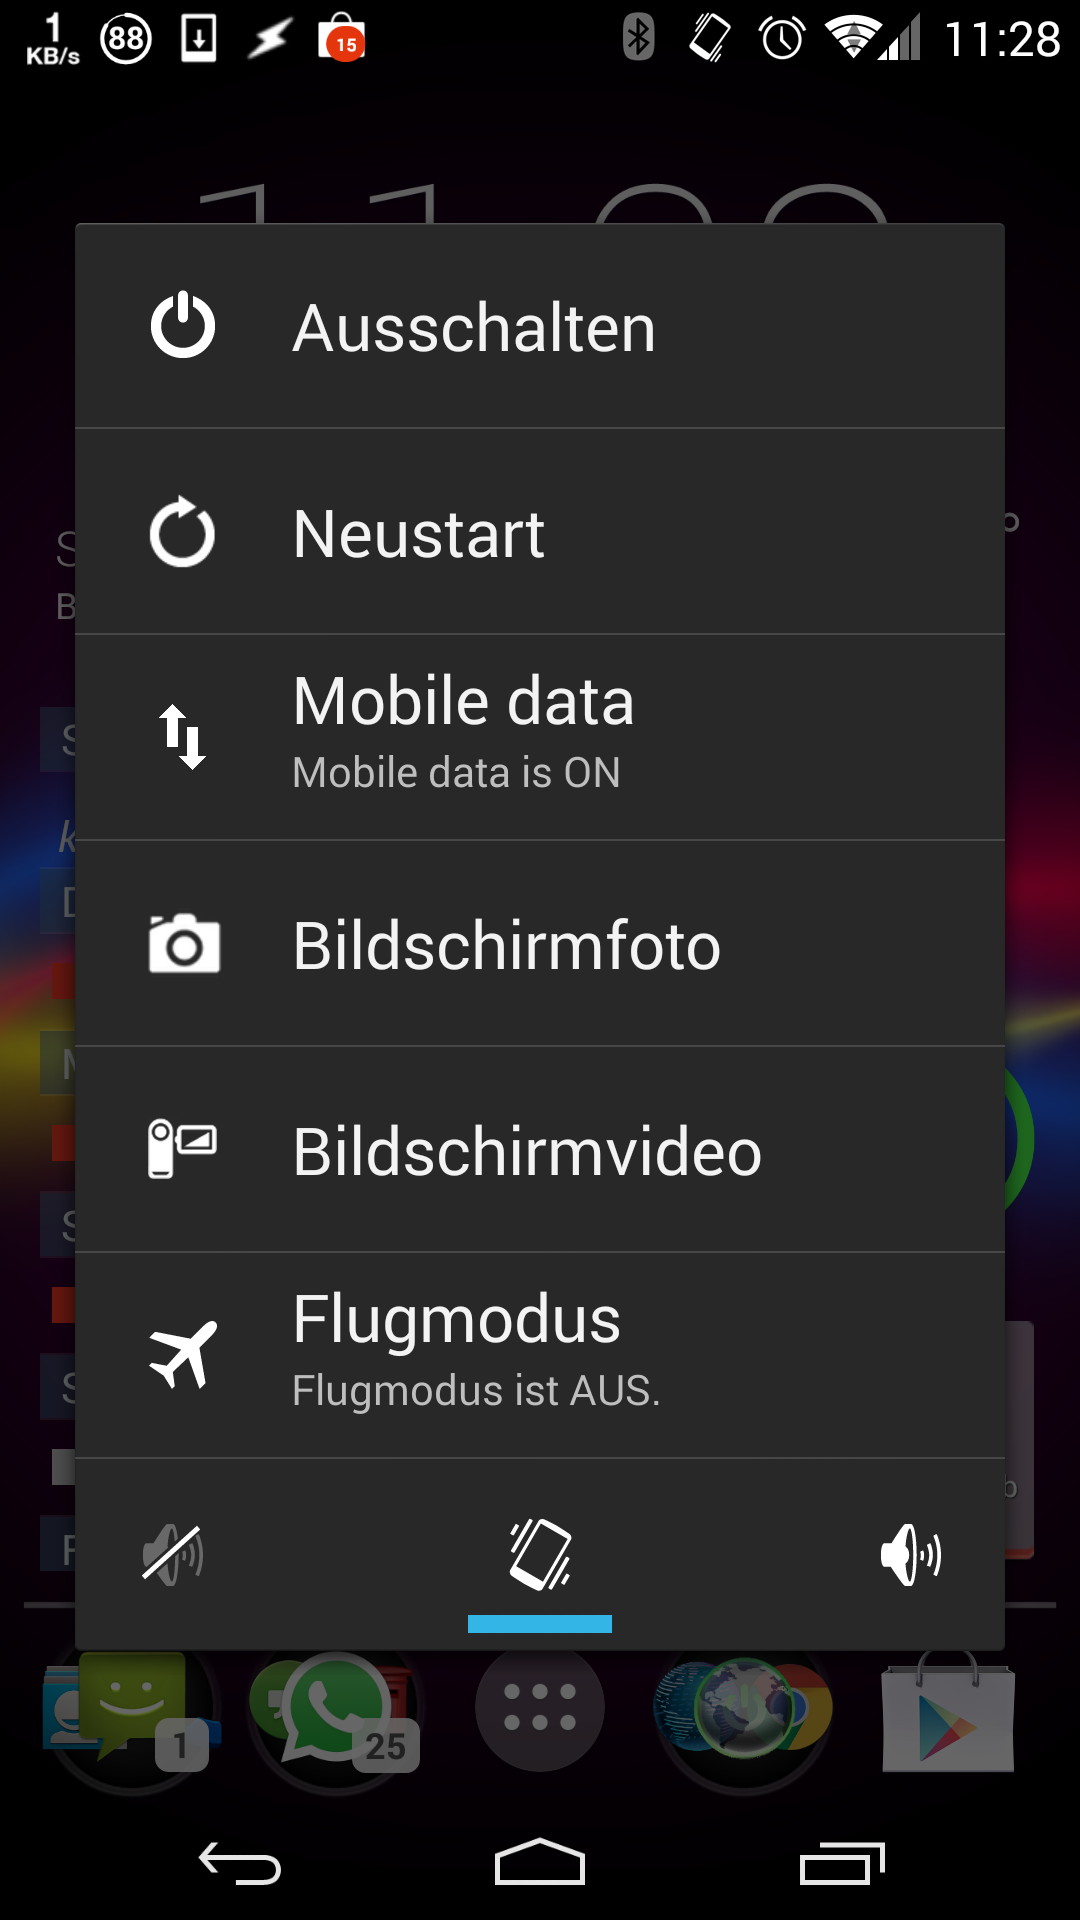
\includegraphics[width=\linewidth]{img/screenshot_omnirom_power_menu}
	\caption{Screenshot des OmniROM Power-Menüs.}
	\label{fig:screenshot_omnirom_power_menu}
\end{wrapfigure}
\ac{ADB} ist ein Debugging-Werkzeug, welches als Bestandteil des Android \ac{SDK} \cite{AndroidOpenSourceProject.2014c} ausgeliefert wird.
Mit ihm lassen sich Befehle direkt auf Shell des Geräts ausführen.
Vor Android 4.4 war es bereits möglich mit dem Befehl \texttt{adb shell screencap -p /sdcard/<name>.png} Bildschirmfotos zu erstellen \cite[vgl.][]{RandomStuff.2013}.
Diese Möglichkeit besteht seit Android 4.0 \enquote{Ice Cream Sandwich} (ICS).

Die beiden genannten Möglichkeiten für Aufzeichnungen des Bildschirminhalts benötigen jedoch einen per \ac{ADB} verbundenen PC.

Um diese Befehle direkt auf dem Gerät aus einer Applikation heraus auszuführen, wird der Root-Zugriff auf dem Gerät benötigt \cite[vgl.][22]{Erxleben.2014}.

Alternativ bieten einige Geräte und sog. \enquote{Custom-ROMs} die Möglichkeit Bildschirmfotos und -videos direkt aus einem Menü heraus oder per Tastenkombination zu erstellen. 
Abbildung \ref{fig:screenshot_omnirom_power_menu} zeigt beispielhaft das Power-Menü von \emph{OmniROM}\footnote{OmniROM Webseite: \url{http://omnirom.org/}}.

Eine Möglichkeit um den Bildschirminhalt auf einem zusätzlichen Display anzuzeigen wird im nächsten Abschnitt kurz erläutert.

\subsubsection{Chromecast Screen Mirroring}
Der Google \emph{Chromecast} ist ein Streaming-Client, welcher z.~B. an Monitoren oder Fernsehern angeschlossen werden kann.
Nach der ersten Einrichtung kann er u.~a. über Android Geräte im selben Netzwerk gesteuert werden.
Applikationen mit \emph{Chromecast} Unterstützung können Medien auf diesem Weg Inhalte direkt auf einem Bildschirm darstellen. \cite[Vgl.][]{Google.2014}
Neben dem Streaming von Medieninhalten aus dem Internet unterstützt die aktuelle \emph{Chromecast} Applikation für Android \cite{GoogleInc..2014} auch das Übertragen des Bildschirminhalts mit sehr geringer Latenz.
Diese Funktion ist allerdings nicht für alle Geräte verfügbar.
Eine Aufzeichnung der Übertragung wird aktuell nicht unterstützt.

Auch wenn es andere Lösungen gibt, um den Bildschirminhalt eines mobilen Geräts zu übertragen, \emph{Chromecast} ist mit 35~\texteuro\xspace \footnote{Preisangabe des Herstellers, Stand: Oktober 2014. Webseite: \url{https://www.google.de/chrome/devices/chromecast/}} einer der preiswertesten Wege, bei dem nur ein Fernseher oder Monitor benötigt wird.
Besonders spannend sind die Möglichkeiten für Labortests, denn die Kamera, welche den Bildschirm abfilmt könnte entfallen und der Testbenutzer kann sich frei im Raum, bzw. in der Reichweite des kabellosen Netzwerks, bewegen.
\pagebreak

\section{Konzept}
\subsection{Anforderungen}
An das Projekt ergeben sich die folgenden Anforderungen:
\begin{compactitem}
	\item  
\end{compactitem}
\pagebreak
\subsection{Architektur}\label{subsec:architektur}

\begin{wrapfigure}{r}{.5\textwidth}
	\centering
	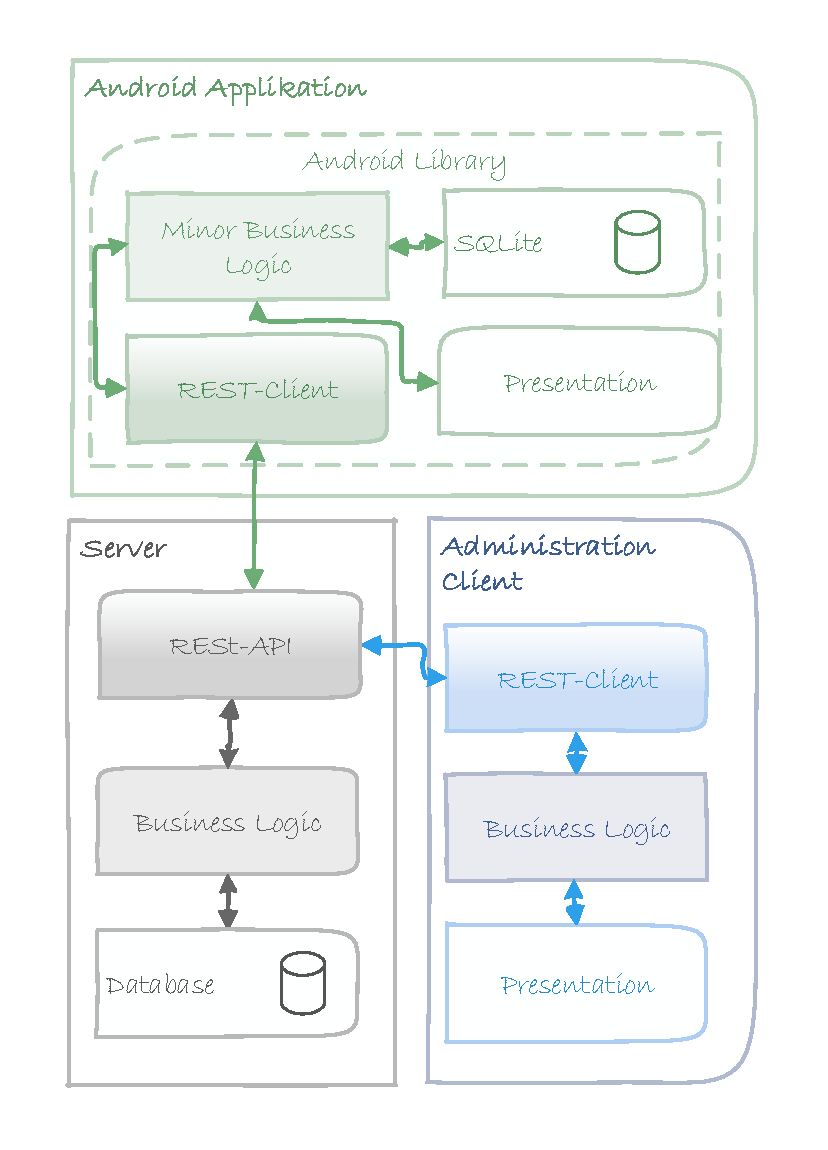
\includegraphics[width=\linewidth]{img/architecture_draft}
	\caption{Architektur des Frameworks.}
	\label{fig:architektur_entwurf}
\end{wrapfigure}
Das Framework ist in drei Komponenten unterteilt: Server, Android Bibliothek und ein Client für Testleiter~/~Administratoren.

Der Aufbau der Komponenten ist in Abbildung \ref{fig:architektur_entwurf} dargestellt.
Die Kommunikation zwischen den Komponenten erfolgt per \ac{HTTP} und ein \ac{REST} - \ac{API}.
Der Server nutzt zur Datenhaltung eine Datenbank, auf welche durch die Geschäftslogik zugegriffen wird.

Der Administrations-Client dient zum Verwalten der Tests, Aufgaben und Benutzer, sowie zum Einsehen von Ergebnissen bereits durchgeführter Testsitzungen.
Er besitzt keine eigene Datenhaltung und erhält sämtliche Daten vom Server über einen \ac{REST}-Client.

Die Android Bibliothek kommuniziert auch über einen \ac{REST}-Client mit dem Server.
Um Testsitzungen auch ohne Internetverbindung oder allgemein der Verbindung zum Server durchführen zu können, speichert die Android Bibliothek Tests, Aufgaben und die gesammelten Daten von Testsitzungen lokal zwischen.
Diese werden bei der nächsten Verbindung mit dem Server an diesen übertragen.
\subsection{Technologien und Werkzeuge}

\subsubsection{Android Bildschirmaufzeichnung}
Eine der Neuerungen, welche mit Android 4.4 \enquote{KitKat} eingeführt wurde, ist die Möglichkeit den Bildschirminhalt in Form eines Videos aufzuzeichnen.
Die Aufzeichnung wird über einen PC gestartet, der mit dem Android Gerät über die \ac{ADB} \cite{AndroidDevelopers.2014b} per \ac{USB}-Kabel oder kabellos verbunden ist.
Die Aufzeichnung wird mit dem Befehl \texttt{adb shell screenrecord} gestartet werden.
Soll ein Teil einer Applikation nicht aufgezeichnet werden, so kann der Entwickler die Aufnahme mit \texttt{SurfaceView.setSecure()} verhindern.
Die Aufzeichnung wird im MP4"~Format auf dem Gerät gespeichert und lässt sich von dort abrufen, z.~B. mit der \ac{ADB} oder über eine \ac{USB} \ac{MTP}.
\cite[Vgl.][]{AndroidDevelopers.2014}
\begin{wrapfigure}{l}{.3\textwidth}
	\centering
	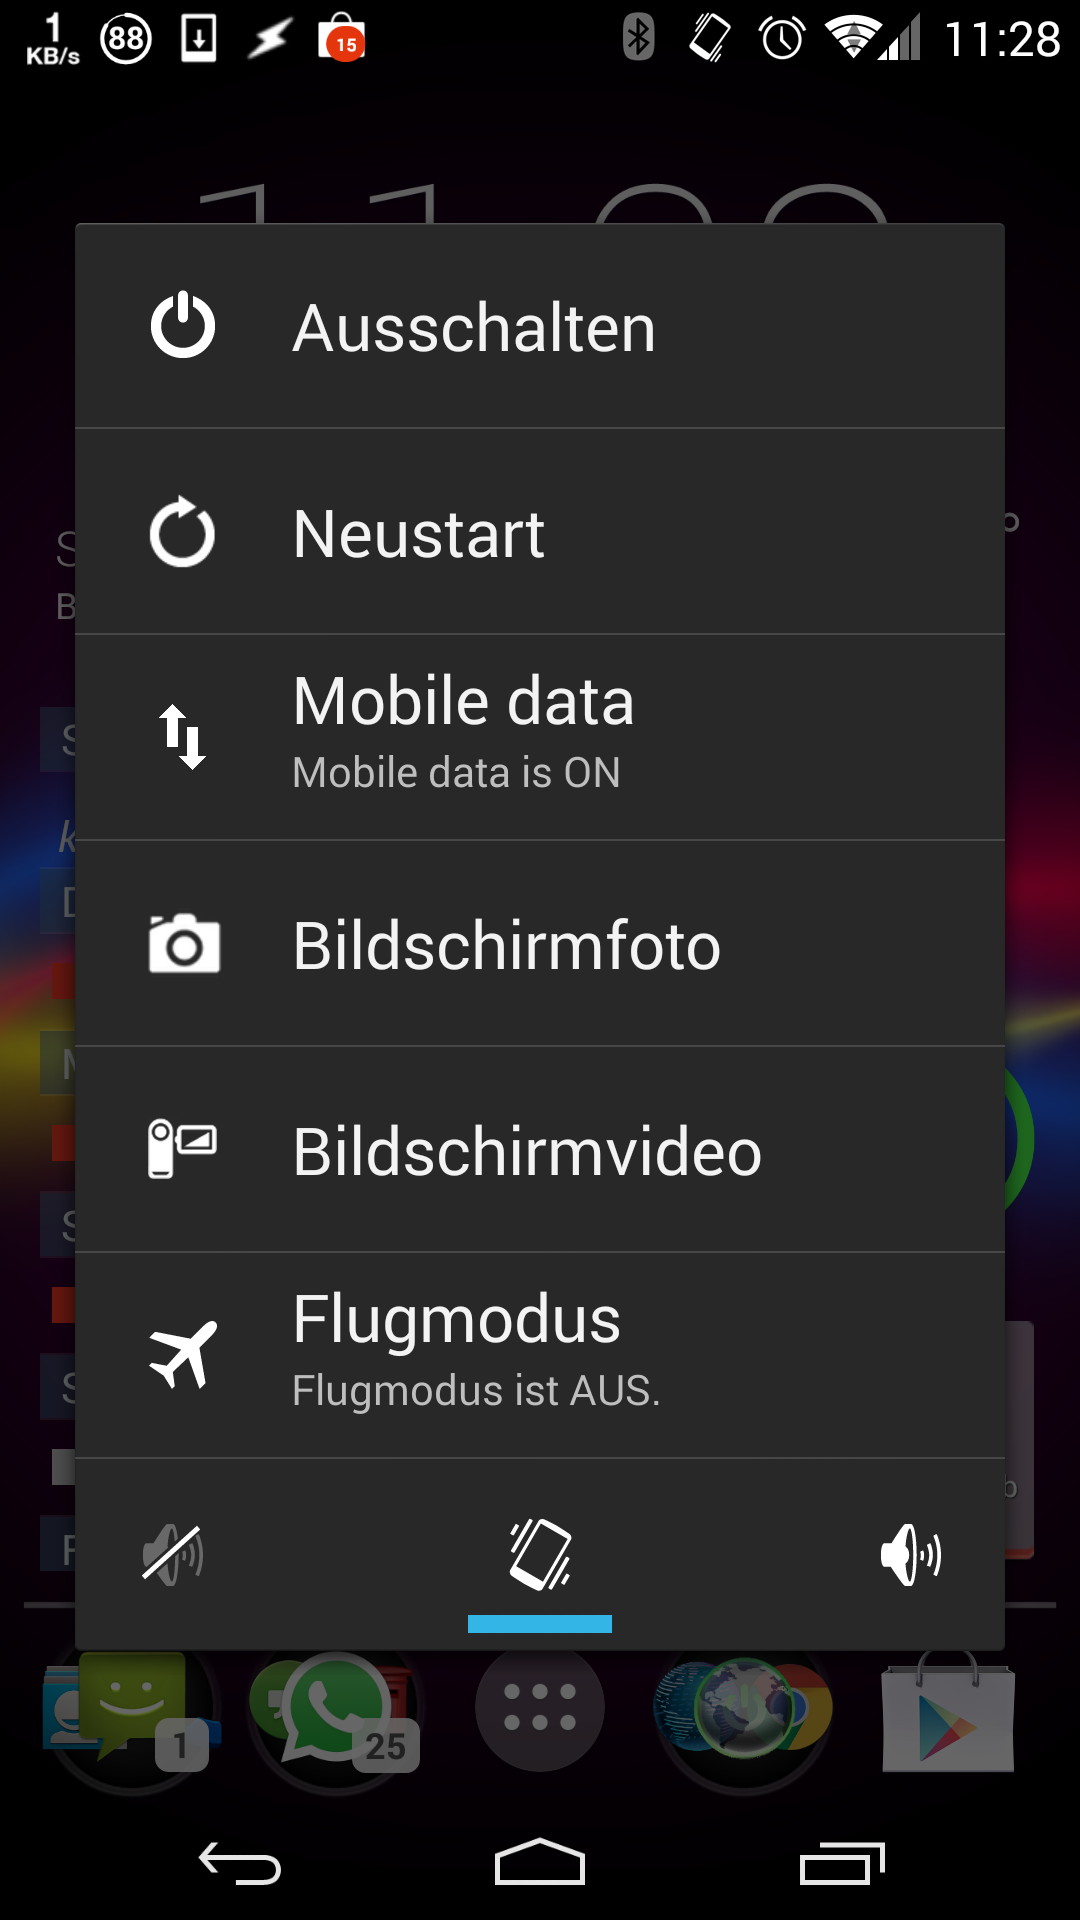
\includegraphics[width=\linewidth]{img/screenshot_omnirom_power_menu}
	\caption{Screenshot des OmniROM Power-Menüs.}
	\label{fig:screenshot_omnirom_power_menu}
\end{wrapfigure}
\ac{ADB} ist ein Debugging-Werkzeug, welches als Bestandteil des Android \ac{SDK} \cite{AndroidOpenSourceProject.2014c} ausgeliefert wird.
Mit ihm lassen sich Befehle direkt auf Shell des Geräts ausführen.
Vor Android 4.4 war es bereits möglich mit dem Befehl \texttt{adb shell screencap -p /sdcard/<name>.png} Bildschirmfotos zu erstellen \cite[vgl.][]{RandomStuff.2013}.
Diese Möglichkeit besteht seit Android 4.0 \enquote{Ice Cream Sandwich} (ICS).

Die beiden genannten Möglichkeiten für Aufzeichnungen des Bildschirminhalts benötigen jedoch einen per \ac{ADB} verbundenen PC.

Um diese Befehle direkt auf dem Gerät aus einer Applikation heraus auszuführen, wird der Root-Zugriff auf dem Gerät benötigt \cite[vgl.][22]{Erxleben.2014}.

Alternativ bieten einige Geräte und sog. \enquote{Custom-ROMs} die Möglichkeit Bildschirmfotos und -videos direkt aus einem Menü heraus oder per Tastenkombination zu erstellen. 
Abbildung \ref{fig:screenshot_omnirom_power_menu} zeigt beispielhaft das Power-Menü von \emph{OmniROM}\footnote{OmniROM Webseite: \url{http://omnirom.org/}}.

Eine Möglichkeit um den Bildschirminhalt auf einem zusätzlichen Display anzuzeigen wird im nächsten Abschnitt kurz erläutert.

\subsubsection{Chromecast Screen Mirroring}
Der Google \emph{Chromecast} ist ein Streaming-Client, welcher z.~B. an Monitoren oder Fernsehern angeschlossen werden kann.
Nach der ersten Einrichtung kann er u.~a. über Android Geräte im selben Netzwerk gesteuert werden.
Applikationen mit \emph{Chromecast} Unterstützung können Medien auf diesem Weg Inhalte direkt auf einem Bildschirm darstellen. \cite[Vgl.][]{Google.2014}
Neben dem Streaming von Medieninhalten aus dem Internet unterstützt die aktuelle \emph{Chromecast} Applikation für Android \cite{GoogleInc..2014} auch das Übertragen des Bildschirminhalts mit sehr geringer Latenz.
Diese Funktion ist allerdings nicht für alle Geräte verfügbar.
Eine Aufzeichnung der Übertragung wird aktuell nicht unterstützt.

Auch wenn es andere Lösungen gibt, um den Bildschirminhalt eines mobilen Geräts zu übertragen, \emph{Chromecast} ist mit 35~\texteuro\xspace \footnote{Preisangabe des Herstellers, Stand: Oktober 2014. Webseite: \url{https://www.google.de/chrome/devices/chromecast/}} einer der preiswertesten Wege, bei dem nur ein Fernseher oder Monitor benötigt wird.
Besonders spannend sind die Möglichkeiten für Labortests, denn die Kamera, welche den Bildschirm abfilmt könnte entfallen und der Testbenutzer kann sich frei im Raum, bzw. in der Reichweite des kabellosen Netzwerks, bewegen.
\pagebreak

\section{Realisierung des Servers\label{sec:realisierung_server}}
\subsection{Datenbank und Persistenz\label{subsec:datenbank}}
Um die gesammelten Daten von den Testsessions, Metadaten, Tests und Aufgaben verwalten und speichern zu können, wird ein \ac{DBMS} verwendet.
Bei der Entwicklung wurde weitgehend darauf geachtet keine herstellerspezifischen Funktionen und Eigenschaften zu verwenden.
Für die Entwicklung wird eine \emph{MySQL}-Datenbank verwendet, welche laut Aussage des Anbieters \enquote{The world's most popular open source database} \cite{OracleCorporation.2014} sei.
Die Datenbank kommt in der quelloffenen \enquote{Community Edition} (\ac{GPL}-Lizenz) in der Version 5.7 zum Einsatz.

Als Abstraktionsschicht wird die \ac{JPA} verwendet, als Provider \emph{EclipseLink}.
Letzterer ist der \ac{JPA} Standardprovider des \emph{Glassfish} \ac{AS}. 

\subsubsection{Konfiguration des Glassfish AS zur Verwendung einer MySQL Datenbank}
Mit dem kostenlos verfügbarem Werkzeug \emph{MySQL Workbench} \cite{Oracle.2014b} wurden zuerst ein Datenbankschema \texttt{hipsterbility} und ein Benutzer \texttt{hipsterbility} angelegt.
Dieser Benutzer erhält volle Zugriffsrechte auf das erstellte Schema.
Da der \emph{Glassfish}-Server und die \emph{MySQL}-Datenbank auf dem selben System betrieben wurden, erhält der Benutzer nur lokale Anmelderechte.
Bei Fernanmeldungen sollte ein starkes Passwort verwendet werden.

Im nächsten Schritt wird der \emph{MySQL}-\ac{JDBC} Treiber in das entsprechende Verzeichnis des \emph{Glassfish}-Server kopiert. Dieser Schritt ist in der Dokumentation \cite{OracleCorporation.2014b} ausführlich beschrieben.



\subsubsection{Datenmodell und Datenbankschema}
Die Datenbank wurde nach dem \enquote{Code first} Ansatz entwickelt.
Diese Vorgehensweise wurde gewählt, da das bisherige Datenmodell erweitert wurde und die Datenbank nach belieben angepasst werden kann, da keine anderen Anwendungen direkt auf die Datenbank zugreifen.

Das Datenmodell besteht aus \ac{JPA}"~Entitätsklassen (Entity). 
Dies sind mit \ac{JPA}"~Annotationen versehene \ac{POJO}-Klassen sind \cite[vgl.][17-19]{Keith.2013}.

Das resultierende Datenbankschema (siehe Abbildung \ref{fig:datenmankschema}) wird durch den \ac{ORM}"~Provider erstellt und bedarf keine manuellen Anpassungen, da Schlüssel, Beziehungen und Einschränkungen der Tabellen direkt in den Entitätsklassen mit Annotationen festgelegt werden können.

Lediglich eine View wurde manuell erstellt, um die Vorgabe des Authentifizierungsproviders zu erfüllen (siehe Abschnitt \ref{subsubsec:anmeldedaten_datenbank})

\begin{minipage}[t]{\textwidth}

\begin{tabu}{|>{\ttfamily}X>{\ttfamily}X>{\small}X[2]|}
\everyrow{\hline}
\hline
\rowfont[l]{\normalfont\bfseries} 
Datenbanktabelle & Entitätsklasse(n) & Beschreibung \\ 
app & TestAppEntity & Eine im System registrierte Applikation die für Test vorgesehen ist \\ 
device & DeviceEntity & Registrierte Geräte der Benutzer \\ 
user & UserEntity & Benutzerdaten und Sammlungen von Objekten mit Benutzerbezug \\ 
realmgroup & GroupEntity & Rollenzuweisung der Benuter \\ 
invite & InviteEntity & Einladung für die Registrierung neuer Benutzer \\ 
session & TestSessionEntity & Repräsentation eines durchgeführten Testdurchlaufs \\ 
test & TestEntity & Objekt zur Darstellung eines Usability-Tests \\ 
task & TaskEntity & Eine Aufgabe in einem Usability-Test, welche vom Testbenutzer ausgeführt werden soll. \\ 
test\_deviceclasses & \emph{DeviceClass} String enum & Eine Liste mit Geräteklassen für die der jeweilige Test durchgeführt werden soll. \\ 
sessionfile & FileEntity \normalfont{Subklassen} & Tabelle mit Pfaden und Metainformationen zu Dateien, die vom Android-Client während einer Testsitzung erstellt werden \\ 

\end{tabu} 
\label{tbl:tabellen_und_entities}
\captionof{table}{Tabellen und Entitäten der Persiszenzschicht.}
\end{minipage}
\subsection{RESTFul Webservice}
Um die Android Bibliothek und den Testleiter-Client anzubinden wird eine \ac{REST}-\ac{API} verwendet.
Da der \emph{Glassfish} \ac{AS} die Grundlage für die Serverkomponente darstellt, kommt die \ac{JAX-RS} 2.0 Implementierung \emph{Jersey} (\url{https://jersey.java.net/}) zum Einsatz, welche beim \ac{AS} mitgeliefert wird.
Als Referenz für die Implementierung der Schnittstelle und den Aufbau der Ressourcen dient \citetitle{Burke.2014} von \citeauthor{Burke.2014} \cite{Burke.2014}.

Eine möglichst lose Kopplung der verschiedenen Klassen wird durch die Verwendung von Interfaces und Dependency Injection erreicht.
Ein gutes Beispiel dafür zeigt Robert Leggett mit seinem GitHub Projekt \emph{jersey\_restful\_webservice}\footnote{GitHub Repository: \url{https://github.com/Robert-Leggett/jersey_restful_webservice}}, welches vom Ressourcenaufbau eher dem \ac{REST}-\ac{RPC} Schema folgt.

Aktuell wird nur das \ac{JSON} Datenformat unterstützt.
Für das (Un--)Marshalling wird serverseitig die \emph{Jackson} (\url{https://github.com/FasterXML/jackson}) Bibliothek verwendet.

Eine Implementierung des \ac{HATEOAS} Prinzips \cite[vgl.][11-13]{Burke.2014} wurde nicht vorgenommen, da die entwickelte \ac{API} nicht öffentlich zugänglich sein wird.
Außerdem wird sie aktuell nur von den eigenen Clients genutzt, welchen der Aufbau der \ac{API} nd Ressourcen bekannt ist.
Ein detaillierte Beschreibung der Ressourcen mit Pfaden und \ac{HTTP}"~Methoden befindet sich in Abschnitt \ref{subsubsec:rest_ressourcen}.

\subsubsection{Java REST-API mit JAX-RS Annotationen und CDI}

\subsubsection{Implementierte Ressourcen\label{subsubsec:rest_ressourcen}}
Die Ressourcen werden als Gruppen von Objekten angesehen und es werden Nomen im Plural verwendet \cite[vgl.][20\psqq]{Burke.2014} um die Benennung einheitlich zu gestalten (z.B. \texttt{users, sessions, devices}).
Dies weicht vom Datenbankmodell ab, da dort die Tabellen im Singular benannt sind (siehe Abschnitt \ref{subsec:datenbank}).

Wie auch bei den \acp{DAO} in der Persistenzschicht der Serveranwendung wurden die vier grundlegenden Datenoperationen \ac{CRUD} implementiert.
Die Zuordnung zwischen Operation und \ac{HTTP}"~Methoden bzw. \ac{SQL}"~Befehlen ist in Tabelle \ref{tbl:crud} zu sehen.

\begin{minipage}[t]{\textwidth}
	\centering
	\begin{tabu}{|X|>{\ttfamily}X|>{\ttfamily}X|}
	\rowfont[l]{\normalfont\bfseries} 
		\hline Operation & HTTP & SQL \\ 
		\hline Create & POST & INSERT \\ 
		\hline Read / Retrieve & GET & SELECT \\ 
		\hline Update / Modify & PUT & UPDATE \\ 
		\hline Delete & DELETE & DELETE \\ 
		\hline 
	\end{tabu}
	\captionof{table}{Zuweisung der CRUD Operationen und HTTP-Methoden und SQL-Befehlen.}
	\label{tbl:crud}
\end{minipage}

\subsubsection{Aufbau von Ressourcen und Zugriffsrechte}
Die Ressourcen sind flach gehalten.
Je nach Benutzerrolle führen Aufrufe der Methoden zu verschiedenen Ergebnissen.
Bei Ressourcen mit Benutzerbezug (z.~B. Geräte und Testsitzungen) bekommt ein angemeldeter Benutzer in der Rolle \texttt{USER} nur Objekte, welche mit ihm in Relation stehen.
Dadurch wird sichergestellt, dass einfache Benutzer nicht auf Daten anderer Benutzer zugreifen können.
Benutzer in der Rolle \texttt{ADMIN} können hingegen auf alle Objekte in einer Ressource zugreifen.

Das erstellen von Objekten mit Benutzerbezug über die \texttt{POST}"~Methode erfordert in der Rolle \texttt{ADMIN} zusätzlich zu dem zu erstellenden Objekt auch noch die \texttt{ID} des Benutzers, für welchen diese erstellt werden soll, sofern die Objekte keine bidirektionale Beziehung haben und sich der Bezug daraus herstellen lässt. 

Nachfolgend werden die Resourcen mit den implementierten \ac{HTTP}"~Methoden aufgelistet.
Die Pfadangabe erfolgt relativ zur Basis"~\ac{URL}.
Angaben in geschweiften Klammern sind Pfad-Parameter, welchen im Aufruf ein Wert zugewiesen ist.
%TODO: fehlende Ressourcen nachpflegen


\begin{minipage}[t]{\textwidth}
	\centering
	\begin{tabu}{>{\ttfamily}X[2]X[1]>{\ttfamily}X[3]>{\small}X[4]}
		\rowfont[l]{\normalfont\bfseries\normalsize}
		Rollen & Methode & Pfad &   Beschreibung\\
		USER & GET & /users &   Daten des angemeldeten Benutzers\\ 
		ADMIN & GET & /users &  Liste aller Benutzer\\
		USER & PUT & /users & Bestätigung oder Fehlermeldung\\
		ADMIN & PUT & /users/\{id\} & Bestätigung oder Fehlermeldung\\ 
		ALL, ADMIN & POST & /users &  ID des neu erstellten Benutzers\\
		ADMIN & GET & /users/\{id\} & Ausgabe des Benutzers mit der ID \texttt{id}\\
		ADMIN & DELETE & /users/\{id\} & Löschen des Benutzers mit der ID \texttt{id}\\
		\\
		USER & GET & /devices & Liste mit Geräten des Benutzers\\
		ADMIN & GET & /devices & Liste mit allen Geräten\\
		ADMIN & GET & /devices/\{id\} & Gerät mit der ID \texttt{id}\\
		
		ADMIN & DELETE & /devices/\{id\} & Gerät mit der ID \texttt{id}\\
		ADMIN & PUT & /devices/\{id\} & Gerät mit der ID \texttt{id}\\
	\end{tabu}
	\captionof{table}{REST"~Ressourcen mit HTTP"~Methoden, Pfad, Benutzerrolle und Beschreibung.}
	\label{tbl:rest_ressourcen}
\end{minipage}



\subsection{Server Sicherheitsmaßnahmen}


\subsubsection{Authentisierung und Autorisierung}



\subsubsection{Speichern von Anmeldedaten in der Datenbank\label{subsubsec:anmeldedaten_datenbank}}
Um die Skalierbarkeit der Anwendung zu gewährleisten, werden die Anmeldedaten der Benutzer in der Datenbank gespeichert.
Das hat den Vorteil, dass der Bezug zwischen Benutzer, Anmeldedaten und weiteren Informationen jederzeit gegeben ist, da keine externen Referenzen verwaltet werden müssen.
Ein Nachteil dieser Vorgehensweise ist jedoch, dass jeder Datenbankbenutzer mit Lesezugriff auf das \emph{hipsterbility}-Schema auf die Benutzerdaten zugreifen kann, wozu auch die Passwörter gehören.
Um diesen Nachteil zu relativieren nutzt der \emph{Glassfish 4} \ac{AS} standardmäßig die kryptografische Hashfunktion \emph{\ac{SHA}-2} mit 256~Bit Hashwerten (\ac{SHA}-256).

Zusätzlich zu der Speicherung der Hashwerte werden die Passwörter durch den Server mit der \emph{\ac{AES}} Blockchiffre verschlüsselt.
Als Passwort zur Ver- und Entschlüsselung wird das \emph{Glassfish} \texttt{Master Password} benutzt \cite[vgl.][16\psq]{OracleCorporation.2013}
Leider ist diese Funktion nur schlecht dokumentiert, es wird zwar grundlegend beschrieben wie ein \texttt{JDBCRealm} eingerichtet wird, jedoch nicht die Bedeutung der einzelnen Sicherheitsparameter \cite[vgl.][50\psq]{OracleCorporation.2013} nicht im Detail erläutert.

\subsection{Authentifizierung mit Java EE Security Realms}
Wie in Abschnitt \ref{subsubsec:anmeldedaten_datenbank} angedeutet, wird für die Verwaltung, Autorisierung und Authentifizierung der Serverkomponente ein \emph{JDBCRealm} eingerichtet.
\emph{Authentication Realms} bilden die Grundlage der Benutzersicherheitsmechanismen im \emph{Glassfish} \ac{AS} und ist Bestandteil von Java EE.
Zu den Hauptfunktionen gehört das Authentisieren, Identifizieren und Autorisieren.

Da für die Datenspeicherung ein \ac{DBMS} verwendet wird, bietet es sich an dort auch die Anmeldedaten der Benutzer zu speichern.

\subsubsection{JDBCRealm Datenbankschema und Entitätsklassen}
Das \texttt{JDBCRealm} sieht dazu ein Schema vor, welches mindestens aus zwei Tabellen besteht (siehe Abbildung \ref{fig:jdbcrealm_minimal_schema}), eine für die Benutzer und eine für Gruppen bzw. Rollen, welche von Benutzern eingenommen werden.
Die Namen der Tabellen und Spalten können bei der Konfiguration angegebene werden und sind entsprechend flexibel.
Benötigt werden eine Tabelle mit Benutzernamen und Passwort (\texttt{Users}) und eine mit der Zuordnung von Gruppenname und Benutzername (\texttt{Groups}).

Bei der Verwendung der \ac{JPA} könnten die zugehörigen Entity-Klassen beispielsweise aussehen, wie in Listings \ref{lst:jdbcrealm_klasse_benutzer} und \ref{lst:jdbcrealm_klasse_gruppe}.

\begin{minipage}[t]{0.5\textwidth}
\begin{lstlisting}[language=Java,caption={Beispiel für eine UserEntity Klasse.}, label=lst:jdbcrealm_klasse_benutzer]
// [...] Imports etc.
@Entity(name = "Users")
public class UserEntity {

    @Id
    private String username;
    private String password;
    // [...] Getter und Setter.
}
\end{lstlisting}
\end{minipage}
\begin{minipage}[t]{0.5\textwidth}
\begin{lstlisting}[language=Java,caption={Beispiel für eine GroupEntity Klasse.}, label=lst:jdbcrealm_klasse_gruppe]
// [...] Imports etc.
@Entity(name = "Groups")
public class GroupEntity {

    @Id
    private int id;
    private String name;

    @ManyToOne
    @JoinColumn(name = "username")
    private UserEntity user;
    // [...] Getter und Setter.
}
\end{lstlisting}
\end{minipage}

Dieses Schema hat allerdings, besonders bei der Verwendung der \ac{JPA} einige Nachteile.
Einerseits verhindert es das einfache Verwenden von numerischen Primärschlüsseln bei der Tabelle \texttt{Users}, da das \texttt{JDBCRealm} in der Gruppentabelle einen Benutzernamen und keine ID erwartet. 
Andererseits kann die selbe Gruppe einem Benutzer mehrfach zugeordnet werden, da keine Beschränkungen vorliegen.

\begin{minipage}[t]{\textwidth}
	\centering
	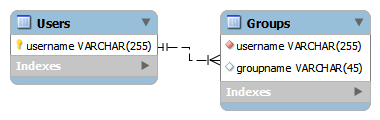
\includegraphics[scale = .75]{img/jdbcrealm_schema}
	\captionof{figure}{Beispielhaftes minimales Datenbankschema für ein JDBCRealm.}
	\label{fig:jdbcrealm_minimal_schema}
\end{minipage}

\subsubsection{Anpassungen bei der Realisierung}

Die Entitätsklassen und folglich auch das Datenbankschema wurde entsprechend der Nachteile angepasst.
Die Anpassungen sind in Listings \ref{lst:jdbcrealm_klasse_benutzer_code} und \ref{lst:jdbcrealm_klasse_gruppe_code} dargestellt.

Um die Verwendung von numerischen Benutzer--IDs zu ermöglichen wurde eine View erstellt, die das erwartete Schema abbildet, siehe Listing \ref{lst:jdbcrealm_view_code}.
Außerdem wurden entsprechende Beschränkungen in den Tabellen eingeführt.
\begin{lstlisting}[language=SQL,caption={SQL Befehl zum erstellen einer View mit Benutzername und Gruppenname}, label=lst:jdbcrealm_view_code]
CREATE VIEW usergroup AS SELECT u.USERNAME, g.NAME FROM USER u INNER JOIN realmgroup g on g.USER_ID = u.ID;
\end{lstlisting}

Da der Benutzername nicht mehr der Primärschlüssel ist, wurde eine Beschränkung eingeführt, um den Benutzernamen in der Tabelle eindeutig zu halten.
Außerdem darf er, nach dem Erstellen, nicht mehr geändert werden und muss einen Wert enthalten.
\begin{lstlisting}[language=Java,caption={Beispiel für eine UserEntity Klasse.}, label=lst:jdbcrealm_klasse_benutzer_code]
// [...] Imports etc.
@Entity(name = "User")
// [...]
public class UserEntity {
	// [...]
    @Id
    @GeneratedValue(strategy= GenerationType.IDENTITY)
    private int id;
    @Column(unique = true, nullable = false, updatable = false)
    private String username;
    // [...]
    @Column(nullable = false) @XmlTransient @JsonIgnore
    private String password;
    // [...] Getter, Setter und weitere Properties.
\end{lstlisting}

Die Gruppen oder Rollentabelle wurde um Beschränkungen erweitert, die eine Mehrfachzuordnung des selben Benutzers zu einer einzigen Gruppe untersagen.
\begin{lstlisting}[language=Java,caption={Auszug aus der GroupEntity Klasse.}, label=lst:jdbcrealm_klasse_gruppe_code]
// [...] Imports etc.
@Entity(name = "RealmGroup")
@Table(uniqueConstraints = @UniqueConstraint(columnNames = {"NAME, USER_ID"}))
public class GroupEntity {
    // [...]
    @Id
    @GeneratedValue(strategy=GenerationType.IDENTITY)
    private int id;
    @Column(nullable=false)
    private String name;
    @ManyToOne
    private UserEntity user;
    // [...] Getter und Setter.
}
\end{lstlisting}

Wenn die nötigen \ac{JDBC}"~Ressourcen bereits erstellt wurde, kann das \texttt{JDBCRealm} mit dem Befehl aus Listing \ref{lst:asadmin_create_realm} mit dem \texttt{asadmin}"~Werkzeug erzeugt werden.
Das Erstellen und Bearbeiten von Realms ist auch über die Weboberfläche möglich, siehe Abbildung \ref{fig:realm_screenshot}.

\subsection{Webservice und REST-API}


\subsection{Server Deployment}
%TODO: Server Deployment
\pagebreak

\section{Realisierung des Testleiter-Clients und der Android Bibliothek}\label{sec:relisierung_client}
\subsection{Realisierung des Clients für Testleiter und Administratoren}
Der Testleiter Client wurde auf Basis von JavaFX mit dem \ac{JDK} 8 erstellt.
JavaFX ist seit Java 8 Bestandteil der Java SE Laufzeitumgebung und unterstützt viele Neuerungen wie Lambda-Methoden und Property-Bindings.
Neben der einfachen \ac{GUI} Entwicklung, wird auch das Rendern von dreidimensionalen Objekten und Szenen mit Hardwarebeschleunigung unterstützt.
Bei JavaFX bietet außerdem Zahlreiche Methoden an um Animationen zu gestalten und Medien wiederzugeben und zu manipulieren.

Das Hauptnachschlagewerk für die Implementierung wird das Buch \citetitle{Dea.2014} von \citeauthor{Dea.2014} \cite{Dea.2014}.

Nachfolgend wir die Erstellung von grafischen Oberflächen in JavaFX kurz beschrieben.

\subsubsection{Grafische Oberflächen mit dem JavaFX Scene Builder 2.0}
Ähnlich der \ac{XML} Layouts bei der Android Plattform, bietet JavaFX die Möglichkeit Oberflächen deklarativ und außerhalb des Quellcodes zu definieren.
Dies geschieht durch \ac{XML} basierte \texttt{FXML}-Dateien.
Um diese nicht manuell erstellen zu müssen, stellt Oracle das Werkzeug \emph{Scene Builder} \cite{OracleCorporation.2014c} zur Verfügung, mit welchen sich Oberflächen im \ac{WYSIWYG} Stil erstellen lassen.

Abbildung \ref{fig:scenebuilder_screenshot} zeigt, den \emph{Scene Builder} mit einer geöffneten \texttt{FXML}-Datei.
Wichtige Elemente für das Erstellen von Oberflächen sind die Zuweisung einer Controller Klasse, die Vergabe der \texttt{fx:id} und bei Schaltflächen oder interaktiven \ac{GUI}"~Elementen die \texttt{On Action} Methode.

Die Möglichkeit eine Controller-Klasse zu vergeben zeigt, dass die Verwendung des \ac{MVC} oder \ac{MVP} Entwurfsmuster vorgesehen, bzw. leicht möglich, ist.  
Bei der Implementierung wurde das \ac{MVP} Entwurfsmuster umgesetzt, welches sich dadurch auszeichnet, dass möglichst wenig Programmlogik im View, der Oberfläche, verwendet wir.
Der Presenter beherbergt einen Großteil der Programmlogik und stellt das Bindeglied zwischen Model und View dar. \cite[Vgl.][74]{Dea.2014}

Wenn ein \ac{GUI}-Element eine zugewiesene \texttt{fx:id} (Abbildung \ref{fig:scenebuilder_screenshot} rechts oben) besitzt, so kann es mit der \texttt{@FXML} Annotation an einer Objektvariable in der zugewiesenen Controller-Klasse direkt injiziert werden.
Dies erleichtert die Entwicklung, da diese Objekte nicht mehr manuell instanziert und der Oberfläche zugewiesen werden müssen.
Das injizieren mit der \texttt{@FXML} Annotation ist auch bei Methoden möglich, denen eine \texttt{On Action} Methode vergeben wird.
Dadurch entfällt das manuelle Zuweisen eines \texttt{ActionListeners}.

\subsubsection{Properties und Binding}
Das neu eingeführte Property-Binding ermöglicht das Verknüpfen von \ac{GUI}-Elementen, teilweise auch als \emph{Node}, \emph{Control} oder \emph{View} bezeichnet, mit Properties, welche in der einfachsten Form Wrapper für primitive Objekte darstellen.

Nachfolgend einige Beispiele für Property-Klassen (\texttt{javafx.beans.property} ) in JavaFX:
\begin{compactitem}
	\item \texttt{SimpleBooleanProperty}
	\item \texttt{ReadOnlyBooleanWrapper}
	\item \texttt{SimpleIntegerProperty}
	\item \texttt{ReadOnlyIntegerWrapper}
	\item \texttt{SimpleStringProperty}
	\item \texttt{ReadOnlyStringWrapper}
\end{compactitem}
Diese Beispiele zeigen einige der Property Klassen, welche in zwei Gruppen eingeteilt werden können, Properties mit Lese-/Schreibzugriff und schreibgeschützte Properties.
Der Hauptvorteil dieser Wrapper-Klassen liegt darin, dass sie sowohl die Schnittstelle \texttt{Obervable}, als auch \texttt{ObservableValue} implementieren und sich mit \texttt{addListener()} \texttt{ChangeListener} und \texttt{InvalidationListener} registrieren lassen.
Dadurch müssen die Werte nicht durch Polling abgefragt werden und die Listener werden bei Ereignissen benachrichtigt.
Die Implementierung der Listener ist durch Java-Klassen, anonyme Klassen oder Lambda-Ausdrücke möglich. \cite[Vgl.][75-79]{Dea.2014}

Ein weitere Eigenschaft von Properties sind Bindings.
Dadurch lassen sich zwei oder mehrere Werte synchron halten, indem Properties an \ac{GUI} Elemente gebunden werden.
Einfache Bindings, bei denen nur die Werte synchronisiert werden, gibt es in zwei Varianten, unidirektional und bidirektional. 
Beim unidirektionalen Binding mit \texttt{bind()} wird die Property aktualisiert, an welcher \texttt{bind()} aufgerufen wurde.
Bei bidirektionaler Wertebindung mit \texttt{bindBidirectional()} werden die Werte in beide Richtungen synchronisiert.
Neben der einfachen Wertebindung gibt es noch weitere Bindings die sich wie boolsche Operatoren oder mathematische Funktionen verhalten. \cite[Vgl.][79-81]{Dea.2014}

Diese werden hier jedoch nicht weiter behandelt. 

\subsubsection{Dependency Injection mit afterburner.fx}
\emph{afterburner.fx} \cite{Bien.2014} ist ein minimalistisches Framework, bestehend aus zwei Java Klassen, welches die beiden Prinzipien \emph{Convention over Configuration} und \emph{Dependency Injection} in JavaFX Anwendungen ermöglicht.
Durch das Befolgen eines vorgegebenen Dateischemas und Packageaufbaus können Views praktisch ohne Code erstellt werden, einzig durch eine \texttt{FXML}"~Datei und eine Klasse die von \texttt{FXMLView} erbt.

Das Vorgegebene Schema sieht für \enquote{MyClass} etwa wie folgt aus:

\dirtree{%
.1 /.
.2 MyClassPresenter.java.
.2 MyClassView.java.
.2 myclass.css.
.2 myclass.properties.
.2 myclass.fxml.
}

Es werden eine \texttt{*View.java} und eine \texttt{*Presenter.java} Klasse erwartet, sowie eine \ac{CSS}"~Datei, für die Gestaltung der View, eine \texttt{*.properties}-Datei mit Key-Value Inhalt, z.~B. für Strings, und die \texttt{FXML}"~Datei für das \ac{GUI}"~Layout erwartet.
Die \texttt{.css} und \texttt{.properties} Dateien benötigen nicht zwingend einen Inhalt, sollten jedoch vorhanden sein.

Neben der vereinfachten Oberflächenerstellung bietet das Framework noch eine zweite nützliche Eigenschaft.
Es erlaubt, ohne weitere Konfiguration, Java EE Annotationen (\texttt{javax.inject.*}) für Dependency Injection zu benutzen, wozu andernfalls Frameworks wie \emph{Google Guice}\footnote{Google Guice Webseite: \url{https://code.google.com/p/google-guice/}}, benötigt würden, die eine umfangreiche Konfiguration verlangen. \cite[Vgl.][]{Bien.2014}

Die Verbindung zum Server wird auch hier über einen \ac{REST}"~Client hergestellt.

\subsubsection{REST-Client}
Als \ac{REST}-Client wird der Client der Jersey 2 Implementierung verwendet.
Für Aufrufe erfolgen fließend und erlauben es unnötige Zuweisungen zu vermeiden, z.~B.
\begin{center}
\texttt{Response r = client.target(getBaseUri()).path(<Pfad>).request().head();}
\end{center}

Aus dem Response Objekt können Objekte mit \texttt{.readEntity()} abgerufen werden, dazu muss der Typ des Abzurufenden Objekts im Aufruf übergeben werden und die Entitäten werden automatisch deserialisert. \cite[Vgl.][113\psqq]{Burke.2014}



\subsection{Weiterentwicklung der Android Bibliothek}
Es wurden die folgenden Änderungen an der Android Bibliothek durchgeführt:

\begin{compactitem}
	\item Anpassen des \ac{REST}-Clients an den neuen Server.
	\item Verwendung geteilter Entitätsklassen zwischen Bibliothek und Server.
	\item Überarbeitung der Bildschirmerfassung und Visualisierung von Eingaben.
	\item Anpassung der Oberfläche an die veränderte Terminologie und kleinere Verbesserungen.
\end{compactitem}

Die Screenshots im Anhang \ref{appendix:android} zeigen einen Teil der Änderungen.
MotionEvents werden nun direkt an die Bibliothek weitergereicht.
Dies führt dazu, dass alle Eingaben registriert werden, auch in Views die diese normalerweise konsumieren und so nicht mehr weitergeben. 
\subsection{Testen der Software}

Die Oberfläche wurde manuell getestet und für den \ac{REST}-Client wurde JUnit verwendet.
Die Android Anwendung wurde ausschließlich manuell getestet.
\pagebreak

\section{Ergebnisse}
\subsection{Server}
Die Arbeit an der Serverkomponente war die umfangreichste am Projekt.
Probleme mit der \emph{Glassfish} Konfiguration und dessen teilweise unzureichende Dokumentation haben sehr viel Zeit in Anspruch genommen.
Das Ergebnis ist ein Server mit Datenbankanbindung und \ac{REST}-API, die weitgehend implementiert wurde.
Einzig Funktionen zum Dateiupload konnten aus Zeitgründen nicht mehr implementiert werden, wodurch die Android Bibliothek die gesammelten Daten nicht hochladen kann und die Daten entsprechend nicht für die Auswertung bereitstehen.

\subsection{Testleiter-Client und Android Bibliothek}
Umgesetzt wurden die Anmeldung und die Benutzerverwaltung.
Die Kommunikation mit dem Server wurde in Ansätzen implementiert, verläuft aktuell jedoch synchron im UI-Thread, was zum Blockieren der \ac{GUI} führt, wenn große Datenmengen abgerufen werden.
Um dies zu verhindern sollte der Datentransfer in JavaFX Tasks nebenläufig durchgeführt werden, dies konnte jedoch in der vorgegebenen maximalen Bearbeitungsdauer nicht mehr umgesetzt werde.

Die Android Bibliothek wurde ein wenig verbessert, bei der Erkennung von Eingaben und Gesten und die Persistenzschicht wurde eingeführt, ist jedoch noch nicht voll implementiert.
Es wurde viel Zeit investiert, um eine bessere Möglichkeit zu finden den Bildschirminhalt zu erfassen, ohne Root-Zugriff das System zu haben.
Dies verlief jedoch weitgehend ergebnislos.
Zwar wäre es möglich eine Systemapplikation zu erstellen, dies würde allerdings die Integration in andere Anwendungen erschweren, da Systemanwendungen eine besondere Signatur erfordern. 

\pagebreak
\section{Fazit}
Die Durchführung des Projekts führte zu vertieftem Wissen über verschiedene aktuelle Technologien.
Dazu gehören ein detaillierter Einblick in Java EE und JavaFX, sowie Konzepte wie z.B. Dependency Injection.
Das ursprüngliche Ziel war die Entwicklung eines funktionsfähigen Frameworks, welches aus zwei neu implementierten und einer angepassten Komponente besteht.
Aufgrund der fehlenden Vertrautheit mit den verwendeten Technologien (JavaFX, Java EE 7) und den teilweise schwer ergründbaren Fehlern, die bei der Entwicklung des Servers auftraten, war der Projektumfang deutlich zu groß angesetzt, für eine alleinige Bearbeitung.
Diese Fehleinschätzung führte dazu, dass das Projektziel nicht in vollem Umfang erreicht wurde.

Jedoch wurde eine brauchbare Grundlage mit verschiedenen Beispielen der hier behandelten Konzepte und Technologien geschaffen, auf der sich aufbauen lässt.
Um dieses Framework fertigzustellen, inklusive Unit-Tests und erweiterter Testanalyse müssten jedoch noch viel Zeit investiert werden, was im Rahmen der Projektbearbeitung nicht möglich wäre.
Da das Thema weiterhin spannend ist und Potential enthält wird die Bearbeitung außerhalb des Rahmens des Projekts weitergeführt.
Im nächsten Abschnitt wird kurz auf mögliche Richtungen zur Weiterentwicklung eingegangen.
\subsection{Weiterentwicklung}
\subsubsection{Integrierte Blickverfolgung}
Projekte wie \emph{Opengazer} \cite{TheInferenceGroup..2009} zeigen eindrucksvoll, dass Eye-Tracking bzw. Gaze-Tracking auch ohne spezielles Equipment möglich ist.
Mit Hilfe einer einfachen Webcam gelang dem Entwicklerteam das Verfolgen von Augenbewegungen und die Visualisierung des Fokuspunktes auf dem Computerdisplay.
Die quelloffene Software benötigt für die korrekte Funktion das Markieren von Referenzpunkten im Gesicht auf dem Kamerabild, sowie eine Kalibrierung des Blickes mit Referenzpunkten auf dem Display.

Ein schwerwiegender Nachteil der aktuellen Version ist allerdings, dass der Kopf mög\-lich\-st still gehalten werden und die Webcam fixiert werden muss.
Selbst wenn die Software auf mobile Betriebssysteme portiert und ausgeführt werden könnte, wäre es nur schwer möglich die zuvor genannten Bedingungen zu erfüllen.
Das Testgerät müsste fixiert werden und auch die Testperson dürfte sich beim Test möglichst wenig bewegen.
Die Qualität der Messungen wäre auch bei perfekten Bedingungen fraglich, da schon kleine Messungenauigkeiten den Wert der Messpunkte stark reduzieren würden, da die Displays von mobilen Geräten sehr viel kleiner sind als bei Desktop-PCs oder Notebooks.

\subsubsection{Blickerkennung mit zusätzlicher Hardware}
Eine alternative zur Blickverfolgung mit der integrierten Kamera von mobilen Geräten könnte \emph{The Eye Tribe} \cite{TheEyeTribe.2014} bieten.
Diese bieten einen kompakten Eye-Tracker für \$99 an.
Die Hardware ist mit 1,9 x 20 x 1,9 cm Ausmaßen sehr kompakt und mit 70 g auch leicht genug für den mobilen Einsatz, zumindest an Tablet"~PCs.
Aktuell ist die Software nur unter Microsoft Windows lauffähig, eine Android Version befindet sich, laut Herstellerwebsite, in der Entwicklung.

Blickverfolgung auf einem Smartphone ohne externe Hardware könnte schon in naher Zukunft möglich sein.
Durch die Verwendung von mehreren Kameras in der Gerätefront kann das \emph{Amazon Fire Phone} \cite{amazon.de.2014} schon jetzt die Perspektive des Bildschirminhalts dynamisch an den Betrachtungswinkel des Benutzers anpassen.
Zwar wird das Eye-Tracking vom aktuellen \emph{Fire Phone \ac{SDK}} (noch) nicht unterstützt, lediglich das Head-Tracking, jedoch ist das Smartphone erst seit kurzem in den U.S.A. verfügbar und der Verkaufsstart in Deutschland steht noch aus (stand September 2014).
Welche Möglichkeiten die zusätzlichen Kameras bieten und ob sich mit ihnen eine präzise Blickverfolgung realisieren lässt wird die Zukunft zeigen.


% ----------------------------------------------------------------------------------------------------------
% Literatur
% ---------------------------------------------------------------------------------------------------------
\renewcommand\refname{Quellenverzeichnis}
\pagebreak
\singlespacing % Einfacher Zeilenabstand
\setlength{\bibitemsep}{12pt} % Größerer Abstand zwischen den Einträgen
\printbibliography
% ----------------------------------------------------------------------------------------------------------
% Anhang
% ----------------------------------------------------------------------------------------------------------
\clearpage
\pagenumbering{Roman}
\setcounter{page}{1}
\lhead{Anhang \thesection}

\begin{appendix}
\section*{Anhang}
\phantomsection
\addcontentsline{toc}{section}{Anhang}
\addtocontents{toc}{\vspace{-0.5em}}

\section{Server Konfiguration}
\subsection{Screenshots}
\begin{minipage}[t]{\textwidth}
	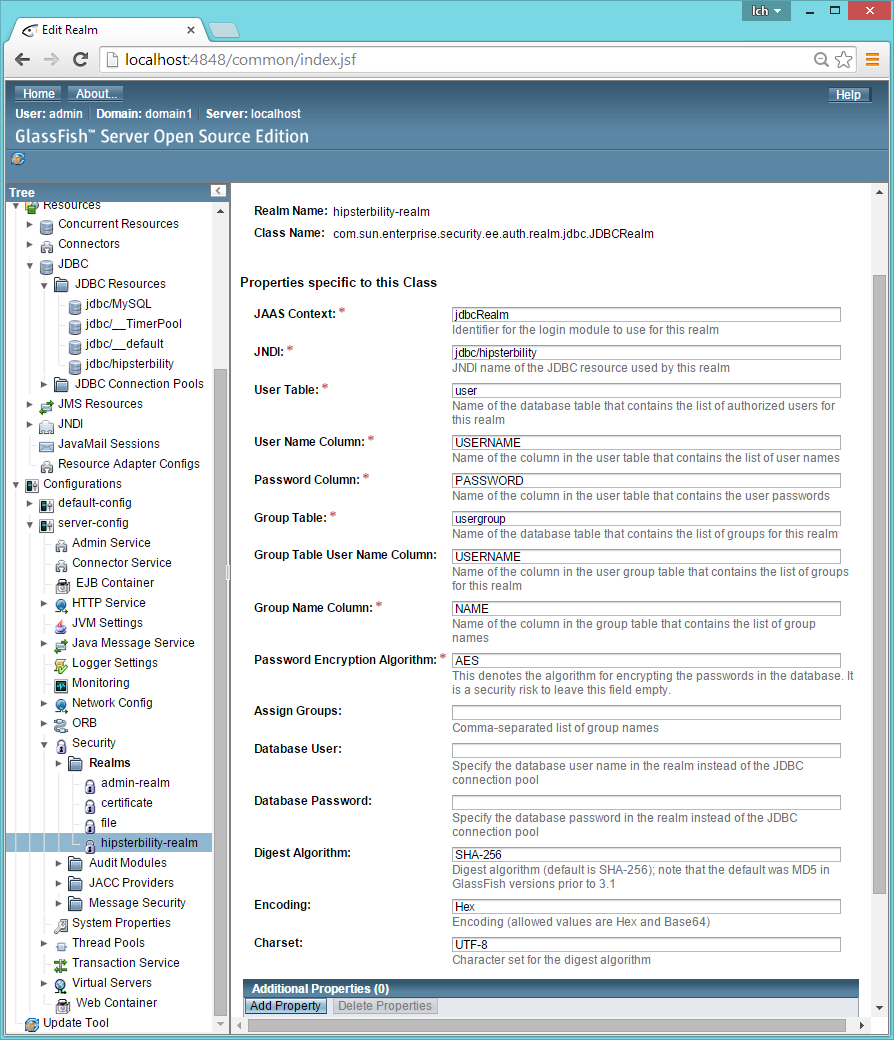
\includegraphics[width = \linewidth]{img/screenshot_realm.png}
	\captionof{figure}{Screenshot der Security-Realm Konfiguration des Glassfish Servers}
	\label{fig:realm_screenshot}
\end{minipage}

\newpage
\subsection{Glassfish Befehle}

\lstinputlisting[caption={Erstellen eines Glassfish Security Realms mit dem \enquote{asadmin} Werkzeug.},language=bash, firstline=2,label=lst:asadmin_create_realm]{../../UsabilityToolkit/HipsterbilityServer/src/main/scripts/glassfish-create.txt}


\subsection{Konfigurationsdateien}

\lstinputlisting[caption={glassfish-resources.xml zum Erzeugen eines JDBC Resource-Pools und einer JDBC Ressource},language=XML,label=lst:glassfish-resources_xml]{../../UsabilityToolkit/HipsterbilityServer/src/main/scripts/glassfish-resources.xml}

\lstinputlisting[caption={glassfish-web.xml JSP Konfiguration und Mapping von SecurityRealm Rollen.},language=XML, label=lst:glassfish-web_xml]{../../UsabilityToolkit/HipsterbilityServer/src/main/webapp/WEB-INF/glassfish-web.xml}

\subsection{Scriptdateien}
\subsubsection{Befehlsdateien}
\lstinputlisting[caption={glassfish-create.txt Befehle zu erzeugen von Ressourcen.},language=bash,label=lst:glassfish-create]{../../UsabilityToolkit/HipsterbilityServer/src/main/scripts/glassfish-create.txt}

\lstinputlisting[caption={glassfish-delete.txt Befehle zum Löschen von Ressourcen.},language=bash,label=lst:glassfish-delete]{../../UsabilityToolkit/HipsterbilityServer/src/main/scripts/glassfish-delete.txt}

\subsubsection*{Windows}
\lstinputlisting[caption={glassfish-create-resources.bat},language=bash,label=lst:glassfish-create-resources_bat]{../../UsabilityToolkit/HipsterbilityServer/src/main/scripts/glassfish-create-resources.bat}

\lstinputlisting[caption={glassfish-delete-resources.bat},language=bash,label=lst:glassfish-delete-resources_bat]{../../UsabilityToolkit/HipsterbilityServer/src/main/scripts/glassfish-delete-resources.bat}

\subsubsection*{Unix / Linux}

\lstinputlisting[caption={glassfish-create-resources.sh},language=bash,label=lst:glassfish-create-resources_sh]{../../UsabilityToolkit/HipsterbilityServer/src/main/scripts/glassfish-create-resources.sh}

\lstinputlisting[caption={glassfish-delete-resources.sh},language=bash,label=lst:glassfish-delete-resources_sh]{../../UsabilityToolkit/HipsterbilityServer/src/main/scripts/glassfish-delete-resources.sh}


\section{Serverkonfiguration}

\lstinputlisting[caption={persistence.xml (Datenbankverbindung)},language=XML, label=lst:persistence_xml]{../../UsabilityToolkit/HipsterbilityServer/src/main/resources/META-INF/persistence.xml}

\lstinputlisting[caption={web.xml (Servlet Konfiguration)},language=XML, label=lst:web_xml]{../../UsabilityToolkit/HipsterbilityServer/src/main/webapp/WEB-INF/web.xml}

\subsection{Diagramme}
\begin{minipage}[t]{\textwidth}
	\centering
	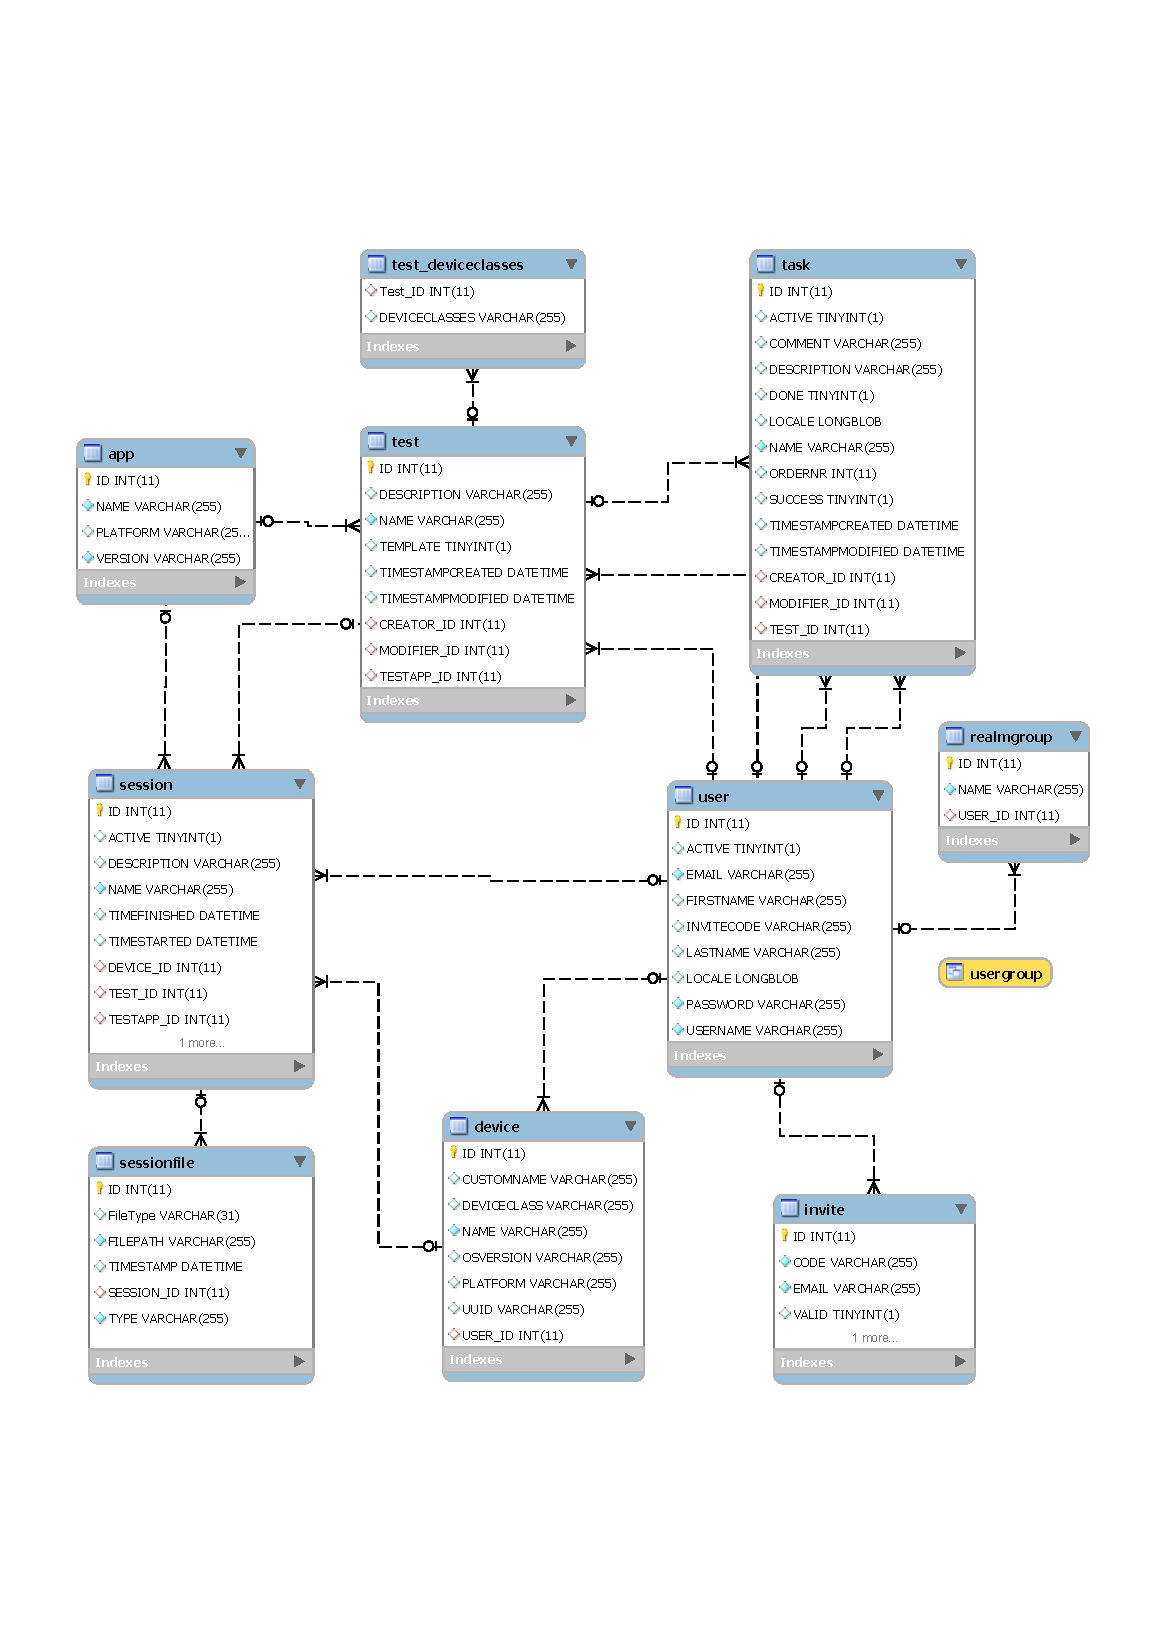
\includegraphics[width=0.95\linewidth]{img/datenbankschema}
	\captionof{figure}{Datenbankschema des Hipsterbility-Servers.}
	\label{fig:datenmankschema}
\end{minipage}
\section{Server Konfiguration}
\subsection*{Screenshots}
\begin{minipage}[t]{\textwidth}
	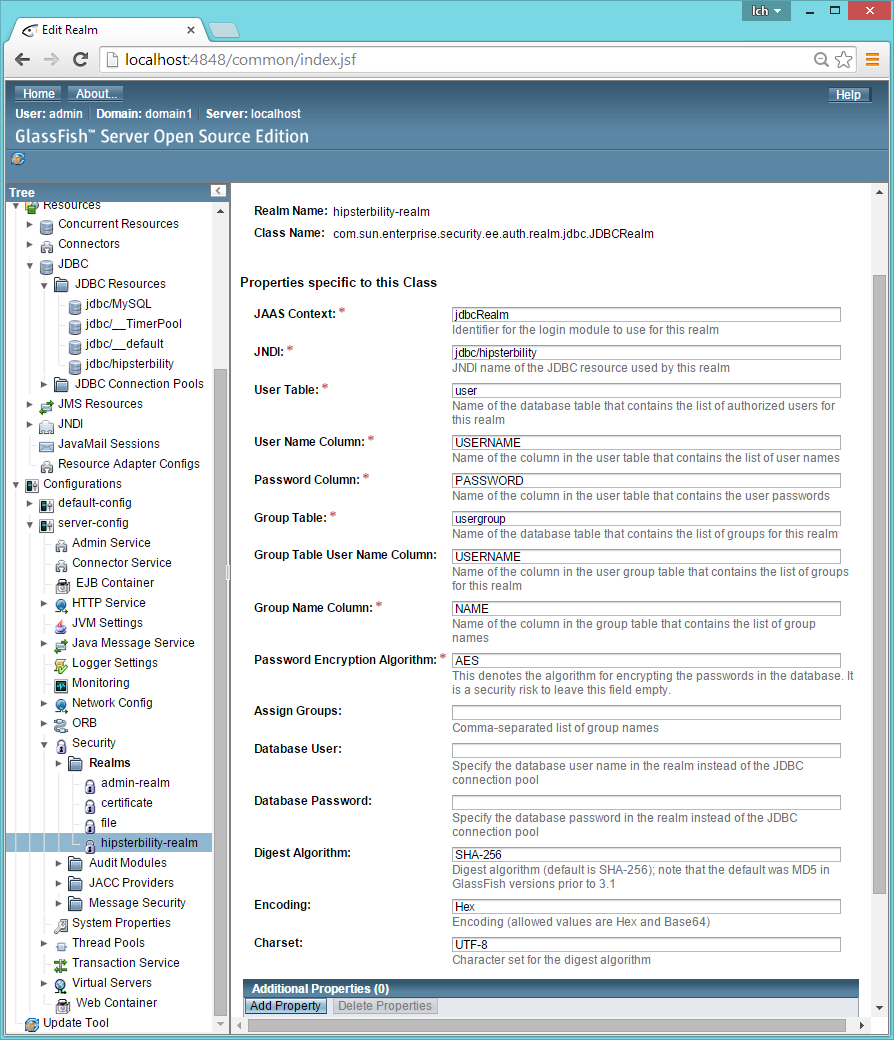
\includegraphics[width = \linewidth]{img/screenshot_realm.png}
	\captionof{figure}{Screenshot der Security-Realm Konfiguration des Glassfish Servers}
	\label{fig:realm_screenshot}
\end{minipage}

\newpage
\subsection*{Glassfish Befehle}

\lstinputlisting[caption={Erstellen eines Glassfish Security Realms mit dem \enquote{asadmin} Werkzeug.},language=bash, firstline=2,label=lst:asadmin_create_realm]{../../UsabilityToolkit/HipsterbilityServer/src/main/scripts/glassfish-create.txt}


\end{appendix}


\newpage
\thispagestyle{empty}
\begin{center}
	\vspace*{5em}
	\huge\textbf{Eidesstattliche Erklärung}\\
\end{center}
\vspace{2em}
Ich erkläre an Eides statt, dass ich die vorliegende Arbeit (entsprechend  der genannten Verantwortlichkeit) selbstständig und nur unter Verwendung der angegebenen Quellen und Hilfsmittel angefertigt habe. Die Arbeit wurde bisher in gleicher oder ähnlicher Form weder veröffentlicht noch einer anderen Prüfungsbehörde vorgelegt.    

\vspace{4em}
\begin{minipage}{\linewidth}
	\begin{tabular}{p{15em}p{15em}}
		Datum: &  .......................................................\\
		& \centering (Unterschrift)\\
	\end{tabular}
\end{minipage}

\end{document}
